\documentclass[a4j, 11pt]{jarticle}
% START:共通設定&共通パッケージ読み込み(基本変更しない)
\renewcommand{\baselinestretch}{1.4}
\setlength{\oddsidemargin}{-0mm}
\setlength{\textwidth}{16cm}
\setlength{\topmargin}{-1.5cm}
\setlength{\textheight}{24cm}
\setlength{\baselineskip}{2cm}
\special{pdf: minorversion=7}    % 出力するPDFのバージョンを指定
\usepackage{ifthen}              % if文制御用
\usepackage[dvipdfmx]{graphicx}
\usepackage{amsmath}             % 数式用
\usepackage{array}               % 数式での場合分け用
\usepackage{url}                 % URL表示用
\usepackage{here}                % [H]用
\usepackage[dvipdfmx]{hyperref}  % 全体像把握&簡易移動のため
\usepackage{pxjahyper}           % 日本語のしおり(ブックマーク)表示用
\hypersetup{pdfborder = {0 0 0}} % hyperrefリンクの囲みを消す
\pagenumbering{roman}            % ページ番号をアラビア数字に変更
\newcounter{fiscal_year}         % 卒業年度計算用
\setcounter{fiscal_year}{\the\year}
\ifthenelse{\the\month < 4}{
	% 年明けから3月までは年-1にする
	\addtocounter{fiscal_year}{-1}
}{}

\usepackage{caption}
\captionsetup[table]{justification=centering}
\captionsetup[figure]{justification=centering}
% END:共通設定&共通パッケージ読み込み(基本変更しない)


% START:ユーザ設定&ユーザパッケージ読み込み---------


% END:ユーザ設定&ユーザパッケージ読み込み-----------


\begin{document}
% START:タイトル
\begin{titlepage}\Large ~
{\normalsize \the\value{fiscal_year} 年度卒業}
\vfill
\begin{center}

% START: 論文の種類-------------------------------
{\Huge 修士論文}
% {\Huge 卒業論文}
% END: 論文の種類---------------------------------
\end{center}
\begin{center}

% START: 日本語タイトル---------------------------
空間解像度差のあるデータセットを用いた深層学習による銀河形状分類精度
% END: 日本語タイトル-----------------------------
\end{center}
\begin{center}

% START: 英語タイトル-----------------------------
日本語タイトル暫定版なため、ここ英語タイトルも未完!
% END: 英語タイトル-------------------------------
\end{center}
\vfill
\begin{center}
\begin{tabular}{|c|l|}
\hline

% START: 論文の種類-------------------------------
所属 & 新潟大学自然科学研究科 電気情報工学専攻・飯田佑輔研究室 \\
% 所属 & 新潟大学工学部情報工学科・林隆史研究室 \\
% END: 論文の種類---------------------------------
\hline

% START: 在籍番号---------------------------------
在籍番号 & F20C026D \\
% END: 在籍番号-----------------------------------
\hline

% START: 論文著者---------------------------------
氏名 & 本間 裕也 \\
% START: 論文著者---------------------------------
\hline
\end{tabular}
\end{center}
\vspace{1cm}
\vfill
\end{titlepage}
\pagebreak
\addtocounter{page}{1}
\thispagestyle{empty}  % このページにページ番号を振らない
% END:タイトル

% START:アブストラクト-----------------------------
\section*{概要}
日本語のアブストラクト

\section*{Abstract}
English Abstract Here

% END:アブストラクト-------------------------------

% START:目次作成
\newpage
\tableofcontents       % 目次作成
\thispagestyle{empty}  % このページにページ番号を振らない
\pagebreak
\pagenumbering{arabic} % ページ番号をアラビア数字に変更
% END:目次作成


% START:本編--------------------------------------
\section{はじめに}

\newpage
\section{深層学習}
\subsection{パーセプトロン}
深層学習の説明を行う前に,

\subsection{ニューラルネットワーク}
ニューラルネットワークとは,

\newpage
\subsection{損失関数と重み更新}
深層学習の学習で用いられる指標を,損失関数と呼ぶ.損失関数には様々な種類が存在し,解く問題の種類によって使い分ける.
一般的な損失関数として,式(\ref{eq:mse})の2乗平均誤差(主に回帰問題に使用) や,式(\ref{eq:ce})のクロスエントロピー誤差(主に分類問題に使用)が挙げられる.

\begin{equation}
	E = \frac{1}{n} \sum_{i=1}^{n} (\hat{y_i} - y_i)^2
	\label{eq:mse}
\end{equation}

\begin{equation}
	E = sans
	\label{eq:ce}
\end{equation}


\newpage
\section{使用するデータセット}
\subsection{Sloan Digital Sky Survey(SDSS)}
\subsubsection*{Sloan Digital Sky Survey (以下,SDSS)について}
SDSS\ref{}とは,天文学史上最も重要なサーベイ観測プロジェクトの一つとも称される大規模プロジェクトである.このプロジェクトは全天の約1/4の天域において,天体の画像および分光データを取得し,天体カタログを作成することを目的としたものである.SDSSでの撮像・分光データ取得はCCDを搭載した地上望遠鏡によって行われる.SDSSの最初のプロジェクトであるSDSS-Iは2000年から2008年まで行われ,また対象を銀河系や超新星に絞ったSDSS-IIプロジェクトが2005年から2008年にSDSS-Iと並行して実施された.その後,太陽系外惑星調査や天の川銀河の構造及び進化などに焦点を当てたSDSS-IIIプロジェクトが2008年から2014年に,南天・北天からの銀河系探索などを目的としたSDSS-IVが2014年から2020年に行われた.

SDSSで撮影された天体のうち低赤方偏移銀河は後述するGalaxy Zooプロジェクトによって形態分類ラベル付けが行われている.SDSSとGalaxy Zooから天体の画像データと分類ラベルを取得できることから,これらのセットを今回の銀河形態分類モデル作成に用いる.
\subsubsection*{銀河画像データの作成方法}
今回分類モデル学習に用いる銀河画像データとして,SDSS-IIプロジェクトにおけるデータリリースの中から,Data Release 7 (以下,DR7)\ref{}より画像データの取得を行った.DR7 を選んだ理由としては,Galaxy Zooプロジェクトにおける銀河形態ラベル付けにDR7の銀河画像が用いられたからである.

データベースから取得できるのはある程度大きな天域の全体画像のため,用いたい銀河の画像を取得したい場合は,全体画像から切り出しを行う必要がある.今回はGalaxy Zooにて形態ラベル付けが為されている銀河の中から15,000天体を対象に,銀河毎に64ピクセル四方のサイズで切り出しを行った.銀河切り出し画像の生成概略図を図\ref{}に示す.

(r-band)DR7におけるデータの撮影が行われたSDSS-IIにおいて,銀河撮像に用いられた測光フィルタはu, g, r, i, zの5つが存在し,これらのフィルタを使用し全可視光域をカバーする5つの帯域画像が撮影された(図\ref{fig:dr7_filters}参照).これら5つの帯域画像のうち,今回の実験ではrフィルタから得られた帯域画像(rバンド画像)を使用している.rバンド画像を使用した理由としては,5つの帯域画像のうち可視光帯画像であるg, r, iバンド画像の中で,最も平均値に近い波長を捉えているrバンド画像がより多くの銀河形態的特徴を有していると考えられること,またrフィルタが5つの測光フィルタのうち最も感度がよいことが挙げられる\ref{}.

\begin{figure}[H]
	\centering
	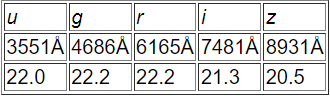
\includegraphics[width=8cm]{images/dr7_filters.png}
	\caption{SDSS Data Release 7 における,銀河撮像に用いられた測光フィルタ一覧\\(フィルタ名,各フィルタによって撮影された画像の波長平均値)}
	\label{fig:dr7_filters}
\end{figure}

\begin{figure}[H]
 \centering
 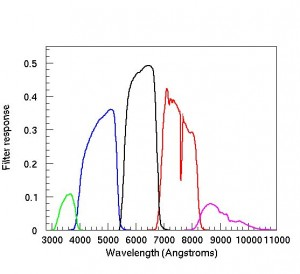
\includegraphics[width=8cm]{images/camera_filters-300x274}
 \caption{SDSSにおける測光フィルタのスループット曲線\\(https://www.sdss.org/instruments/camera/ より引用)}
 \label{fig:filter_responces}
\end{figure}



\subsection{Galaxy Zoo 1 (GZ1)}

\newpage
\section{SDSS \& Galaxy Zooを用いた分類モデル学習}

\newpage
\section{空間解像度差のあるデータセットを用いた分類モデル学習}

\newpage
\section{議論}
\subsection{今回の実験から得た結論}
\subsection{将来課題}
\subsection{将来展望}

\newpage
\section{おわりに}


% END:本編----------------------------------------

% START:参考文献----------------------------------
%% ベタ打ちの場合
% \begin{thebibliography}{1}
% \bibitem{key1}サイト名\\ \url{http://google.com} (yyyy年mm月dd日アクセス) % ウェブサイトの場合
% \bibitem{key2}著者,書籍タイトル,出版                                      % 書籍,論文の場合
% \end{thebibliography}


%% bibtexを使用する場合
\newpage
\bibliography{Master_thesis_bib}         % .bibファイルから拡張子を外した名前 ex)ref.bib
\bibliographystyle{junsrt} % 参考文献出力スタイル
\nocite{*}                 % 参照していない項目も出力する
% END:参考文献------------------------------------


\newpage
\section*{謝辞}
本研究を進めるにあたり,ご指導を頂いた飯田佑輔准教授に厚く感謝申し上げます.
また,日常の議論を通じて多くの知識や示唆を頂いた飯田佑輔研究室の皆様に感謝いたします.

SDSSおよびSDSS-IIの資金はアルフレッド・P・スローン財団から提供され,また参加機関は米国科学財団,米国エネルギー省,米国航空宇宙局,日本の文部科学省,マックスプランク協会,英国高等教育基金協会です.SDSSのWebサイトは、http://www.sdss.org/ です。 

SDSSは参加機関のための天体物理学研究コンソーシアムによって運営されています。参加機関は、アメリカ自然史博物館、ポツダム天体物理学研究所、バーゼル大学、ケンブリッジ大学、ケース・ウェスタン・リザーブ大学、シカゴ大学、ドレクセル大学、フェルミラボ社、高等研究所、日本参加グループ、ジョンズ・ホプキンス大学、原子核宇宙物理学合同研究所、カブリ粒子宇宙物理学研究所、韓国科学者グループ、中国科学者グループ、中国科学者グループ、韓国科学者グループ 韓国科学者グループ、中国科学院(LAMOST)、ロスアラモス国立研究所、マックスプランク天文学研究所、マックスプランク天体物理学研究所、ニューメキシコ州立大学、オハイオ州立大学、ピッツバーグ大学、ポーツマス大学、プリンストン大学、米国海軍天文台、ワシントン大学です.

\end{document}
%------------------------------------------------
